\chapter{Theory}\label{chapter:theory}

\section{Neural network}

Inspired from the nature, neural networks try to imitate the function of human brains. Deep Learning is a specific branch of machine learning. Due to modern technologies like IoT gigantic amounts of data are recorded and processed in order to make production more efficient and reliable. The increased amount of data and computational power makes Deep Learning applications more and more popular. Neural networks are hierarchically structured non-linear processing layers which try to learn hierarchical representations of data. Due to the increasing interest the deep learning community recently came up with various new deep learning architectures. In the following some of those are explained more in detail

\subsection{Neural Network Architecture}
Neural networks consist of neurons which are layered in a hierarchical architecture. The neurons of consecutive layers are connected through weights and biases. During the optimization of the model the weights and biases are updated. Fig. \ref{fig:neural_network_overview} gives an overview of how neurons are arranged in a fully-connected layered architecture. Each neuron from layer i is connected with all neurons from layer i+1 and shares information with them.

\begin{figure}[htpb]
  \centering
  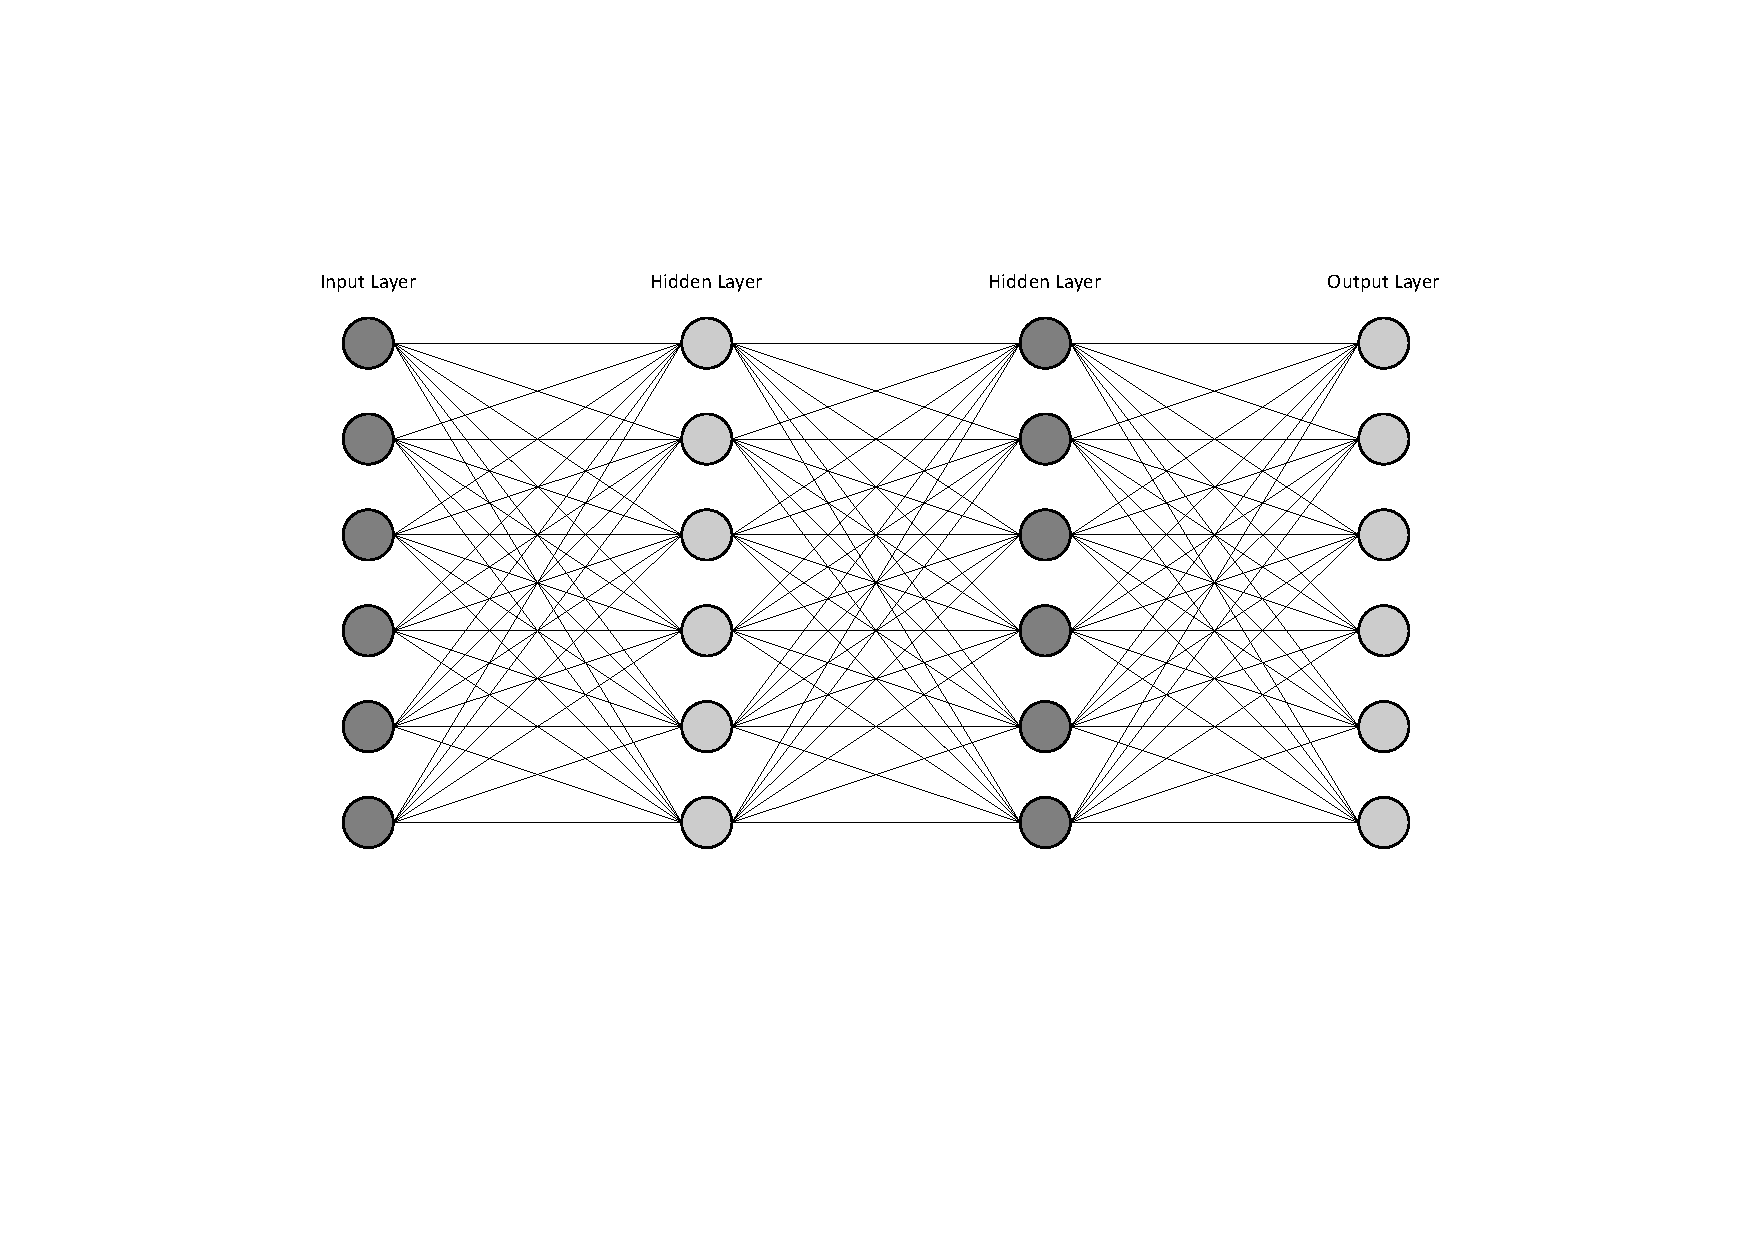
\includegraphics[width=0.7\textwidth, angle =-90]{neural_network_overview.pdf}
  \caption {Layer overview neural network}
  \label{fig:neural_network_overview}
\end{figure}

The input of a neuron is calculated from the sum of all previous neuron's outputs and one bias. Afterwards an activation function is applied to give the neural network a non-linear property. Standard multilayer feedforward networks with even one single hidden layer and an arbitrary bounded and non-constant activation function are universal approximators. This means that a wide variety of functions can be represented by the neural network when given appropriate weights \cite{HORNIK1991}. Without activation functions neural network could only make linear assignments of inputs x to outputs y. With rising data complexity the demand for a "non-linear" mapping from x to y is increasing. Without a non-linearity the neural network with several hidden layers can just learn the same functions as those with just one hidden layer. Such a neural network would not be able to mathematically realise complex relationships in the data. Fig. \ref{fig:neural_network_optimization} shows the forward- and backwardpropagation in a neural network at the example of one single neuron. First the outputs of the neurons $i$ from the previous layers $l-1$ which are connected with the neuron of interest $j$ in layer $l$ are summed up together with a bias $b_{j}$. The resulting logits $z_{j}$ are then processed by the activation function $\phi$. Different activation functions can be used throughout the network. After passing several consecutive hidden layers a loss function evaluates the prediction with the ground truth label in the end of the network.

\subsection{Activation Function}
Different problems and network layers require different activation functions. Typical activation functions are tanh, sigmoid and ReLU in the hidden as well as linear, logistic (sigmoid) and softmax in the final layers of the network \cite{Brownlee2021}. Linear final layers are used for regression problems, whereas sigmoid and softmax functions are typical for classification problems. The sigmoid function is used for binary and softmax for multiclass classification. In general the softmax function is an extension of the sigmoid function to the multiclass case, which can be proofed easily. The softmax and sigmoid functions normalize the network output to a probability distribution over the predicted output classes.  Deciding for the activation functions in the hidden layers is a little more difficult. All just mentioned functions have different characteristics which lead to individual advantages and disadvantages. The sigmoid and tanh function look pretty similar. Both squeeze the inputs in values between -1 and 1. Both functions can suffer from the vanishing gradient problem since the derivative of these functions is close to zero for very big or small inputs. A solution for that is the ReLU function which solves that problem but is limited due to the mapping of negative inputs to zero (dead ReLU) \cite{Brownlee2021}. In the following some of the most used activation functions are described.

\subsubsection{ReLU}

\begin{equation}
ReLU(z) = \lambda
\left\{
\begin{matrix}
0 \quad , if \enspace z < 0\\
z \quad, if \enspace z > 0 \qquad \cite{Nwankpa2021}.
\end{matrix}
\right.
\label{eq:relu}
\end{equation}

\vskip 0.4in

\begin{minipage}{\linewidth}
\makebox[\linewidth]{
  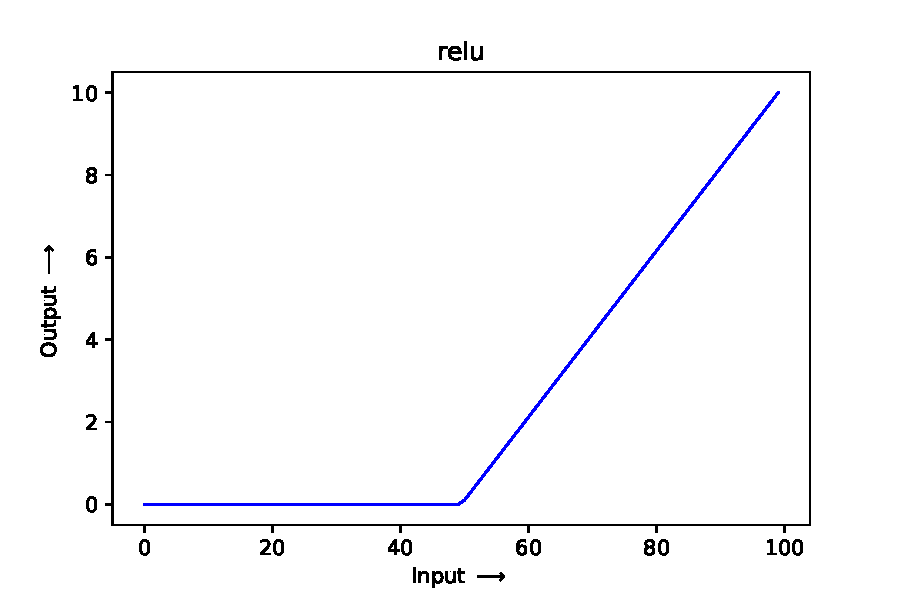
\includegraphics[keepaspectratio=true,scale=0.6]{Activations/relu.pdf}}
\captionof{figure}{ReLU Functions}\label{fig:activations_relu}  
\end{minipage}

\vskip 0.4in

\subsubsection{Sigoid and Softmax}

\begin{equation}
Sigmoid: \sigma(z) = \frac{1}{1+e^{-z}} \qquad \cite{Nwankpa2021}.
\label{eq:sigmoid}
\end{equation}

\begin{equation}
Softmax: \sigma(z)_{i} = \frac{e^{-z_{i}}}{\sum_{j=1}^{K}e^{-z_{j}}} \qquad \cite{Nwankpa2021}.
\label{eq:softmax}
\end{equation}

\vskip 0.4in

\begin{minipage}{\linewidth}
\makebox[\linewidth]{
  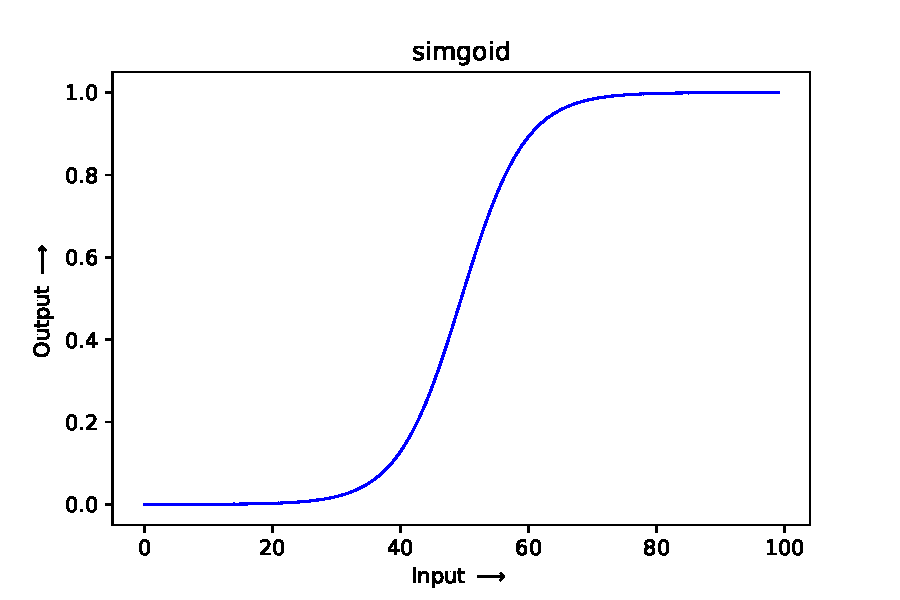
\includegraphics[keepaspectratio=true,scale=0.6]{Activations/sigmoid.pdf}}
\captionof{figure}{Sigmoid Functions}\label{fig:activations_sigmoid}  
\end{minipage}

\vskip 0.4in

\subsubsection{Tanh}

\begin{equation}
tanh(z) = \frac{e^{x}-e^{-x}}{e^{x}+e^{-x}} \qquad \cite{Nwankpa2021}.
\label{eq:tanh}
\end{equation}

\vskip 0.4in

\begin{minipage}{\linewidth}
\makebox[\linewidth]{
  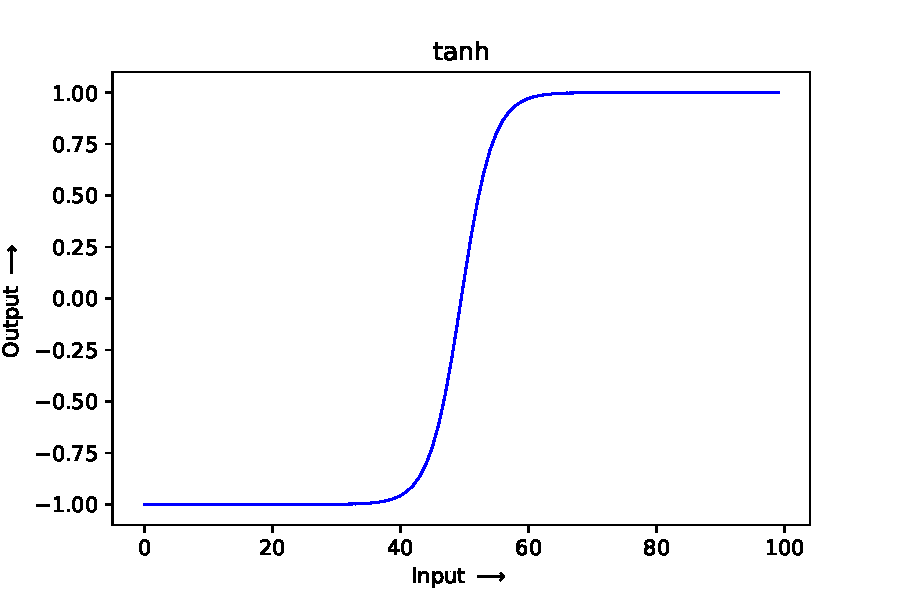
\includegraphics[keepaspectratio=true,scale=0.6]{Activations/tanh.pdf}}
\captionof{figure}{Tanh Functions}\label{fig:activations_tanh}  
\end{minipage}

\subsection{Optimization}
When training neural networks one has to decide for a loss function and an optimizer. 

\subsubsection{Loss}
The loss function acts as a model evaluation criterion and the optimizer is responsible for adapting the model accordingly. Deep Learning models can be divided into two groups: (1) regression tasks and (2) classification tasks. In a regression problem the goal is to learn a mapping function from input variables to a continuous output variable. Contrairwise, in a classification problem the model aims to predict the class label from the input variables \cite{ShilohPerl2020}. Typically Mean Square Error (MSE) , shown in eq. \ref{eq:MSE} , is used for regression problems:

\begin{equation}
L(X) =  \sum_{x}(\hat{y}(x)-y(x))^2
\label{eq:MSE}
\end{equation}

where $y(x)$ is the ground truth and $\hat{y}(x)$ the predicted class label \cite{ShilohPerl2020}. The Cross Entropy Loss, shown in eq. \ref{eq:CE} is rather more used for classification problems: 

\begin{equation}
L(X) = \sum_{x} y(x) log(p(x))
\label{eq:CE}
\end{equation}
where p(x) is the predicted probability of the sample $x$ belonging to the ground truth class $y(x)$ \cite{ShilohPerl2020}.

\subsection{Training Loop}
The weights and biases of the model are adapted such that the loss is minimized. This optimization takes place in a two stage process: (a) feed-forward pass of the input data throughout the model and calculating corresponding neuron outputs and the loss from the predicted and ground-truth labels; followed by (b) backward pass of the loss throughout the model and updating the model weights accordingly. Iteratively this process is performed to optimize the model performance. During the backward pass the gradients of the loss with respect to the network weights is calculated and used to update the weights and biases of the network. The process is visualized in fig. \ref{fig:neural_network_optimization} (green: forward pass, red: backward pass). All the weights and biases are updated recursively by calculating the gradients of every layer, starting from the final and ending at the input layer. Using the chain rule, different partial derivatives of the network can be concatenated. Eq. \ref{chain_rule} shows the chain rule used during backpropagation:
\begin{equation}
 \frac{\delta L_{i}}{\delta w_{i}} = \frac{\delta L_{i}}{\delta \hat{y_{i}}} * \frac{\delta \hat{y_{i}}}{\delta z_{i}} * \frac{\delta z_{i}}{\delta w_{i}}, 
 \label{chain_rule}
\end{equation}
where $\frac{\delta L_{i}}{\delta \hat{y_{i}}}$ is the derivative of the loss with respect to the output of the activation function of the last layer, $\frac{\delta \hat{y_{i}}}{\delta z_{i}}$ is the derivative of the activation function and $\frac{\delta z_{i}}{\delta w_{i}}$ is the derivative of the logits $z_{i}$ with respect to the weights and biases \cite{ShilohPerl2020}.

\begin{figure}[htpb]
  \centering
  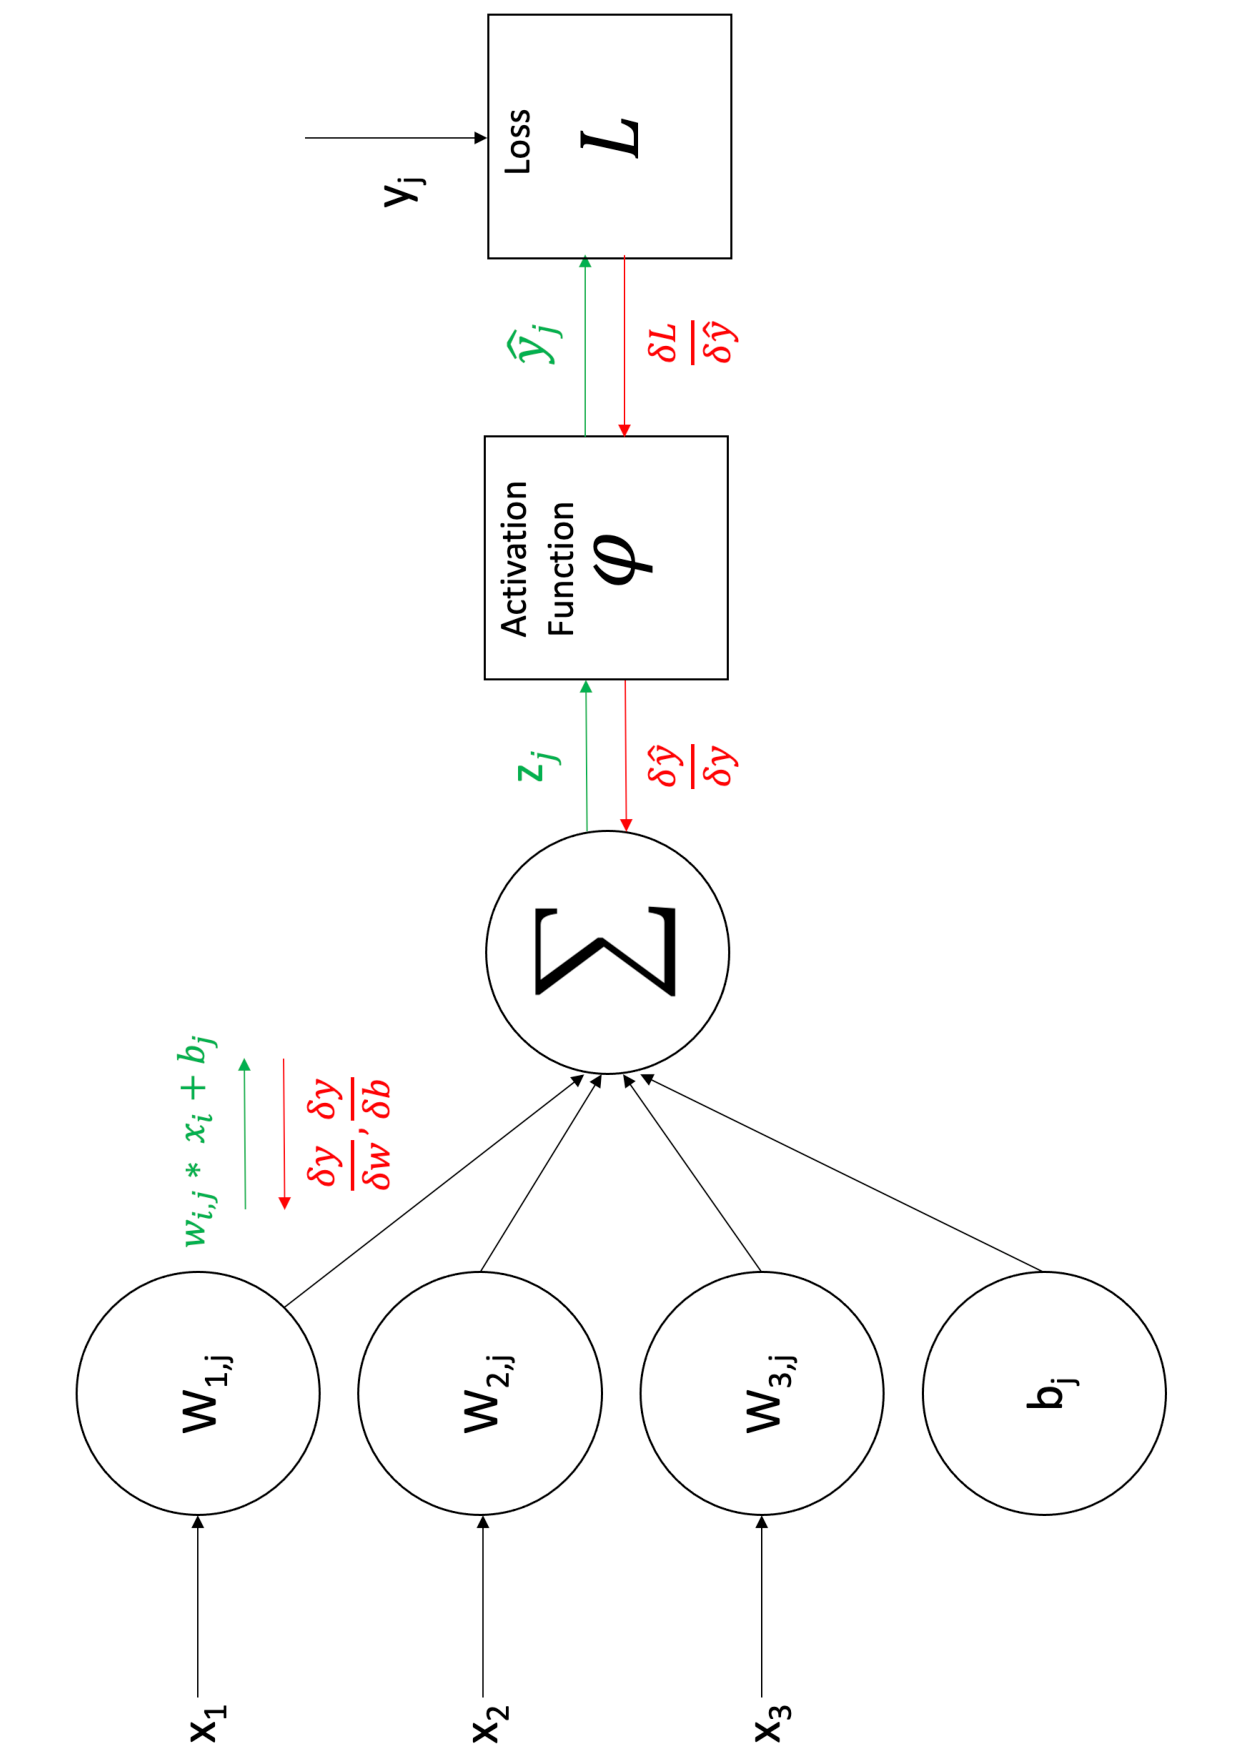
\includegraphics[width=0.7\textwidth, angle = -90]{neural_network_optimization.pdf}
  \caption {Optimization of neural network}
  \label{fig:neural_network_optimization}
\end{figure}


\subsection{Optimizer}
Calculating the gradient for the whole dataset is computationally expensive. A common practice is therefore to separate the dataset in several subsets, so called mini-batches. For each mini-batch the corresponding gradients are calculated and the model is updated accordingly. This process is repeated for all the mini-batches retrieved from the dataset. Each cycle of training over the whole dataset is called an epoch and in every cycle. When the loss converges the training can be terminated. Despite convergence an optimal solution is not assured since the most neural network problems are not convex \cite{ShilohPerl2020}.


Applying gradient descent based optimizer, the weights and biases are updated with a step in the negative direction of the derivative:

\begin{equation}
  w_{new} = w_{old} - \eta \frac{\delta L}{\delta w_{old}},
\end{equation}
where $w_{old}$ are the old, $w_{new}$ are the new model parameters, $\eta$ is the learning rate and $\frac{\delta L}{\delta w_{old}}$ is the derivative of the loss with respect to the current model weights \cite{ShilohPerl2020}. 
Most optimizer rely only on the gradients (first order methods). Using second-order methods do generally converge faster but also require the computation of the Hessian. This is especially expansive for big datasets and models. For this reason Stochastic Gradient Descent is an optimization option which randomly picks samples to optimize the model. For this reason Stochastic Gradient Descent (SGD) is used, which calculates the gradient for single randomly picked samples from the dataset. Since the choice of these samples is random, the optimization suffers from instability and fluctuation. Instead of regular SGD one can use mini-batch gradient descent. This is a compromise between the regular SGD and gradient descent method. The gradient and model update is neither performed for a single sample nor for the whole dataset, but it is performed on a small randomly picked subset of the dataset, which accelerates the convergence of the training.\newline
\newline
In order to accelerate and stabilize the optimization even more one can also include historical gradients. First and second Momentum is a method that helps accelerate SGD in the relevant direction and dampens oscillations \cite{ShilohPerl2020} . Instead of updating with a fixed stepsize in the direction of the negative gradient one can use first and second momentum to adapt the stepsize of the optimization in the different dimensions. In the following four different optimizer which use first, second momentum or a combination of those. An optimization with first momentum works as follows:

\begin{equation}
  \begin{aligned}
  v_{t} = & \gamma v_{t-1} +  \eta \nabla_{\theta}L(W_{t-1}) &\\
  W_{t} = &W_{t-1} - v_{t},
  \end{aligned}
  \label{eq:moment}
\end{equation}

where $M_{t}$ is the momentum, which calculates a moving average over the past gradients, $\nabla_{\theta}L(W_{t})$ is the derivative of the loss with respect to the current model weights, $\beta$ defines the relationship between current gradient and momentum in the moving average, $W_{t-1}$ are the current and $W_{t}$ the updated model weights \cite{Ruder2016}.\newline
\newline
Another well known optimizer of this kind is Nesterov accelerated gradient (NAG) which works just like described in  \ref{eq:moment}. The only difference is that that the gradient is not estimated for the current, but for some pre-udpated model weights. In a first step the gradient is calculated for the old model weights, which are updated with the momentum from the previous iteration $\nabla_{\theta}L( W_{t-1} - \gamma v_{t-1})$. In a second step the current model weights  are updated with the moving average of the momentum and gradient as described in \label{eq:moment} \cite{Ruder2016}.\newline
\newline
Instead of using first momentum, Adagrad builds a moving average of the the past squared gradients (second momentum):

\begin{equation}
  \begin{aligned}
  W_{t} = W_{t-1} - \frac{\eta}{\sqrt[2]{G_{t}+ \epsilon}} \bigodot \nabla_{\theta}L(W_{t-1}),
  \end{aligned}
  \label{eq:Adagrad}
\end{equation}

where  $W_{t-1}$ are the current and $W_{t}$ the updated model weights, $\nabla_{\theta}L(W_{t})$ is the derivative of the loss with respect to the current model weights, $G_{t}$ is second momentum and $\epsilon$ denotes a small quantity which prevents the division by zero  \cite{Ruder2016}.\newline
\newline
The Adaptive Moment Estimation (Adam) is one of the most popular optimizer. ADAM combines the idea of first and second momentum: 
\begin{equation}
  \begin{aligned}
   &m_{t} =  \beta_{1} m_{t-1} +  (1-\beta_{1}) \nabla_{\theta}L(W_{t-1}) &\\
    &v_{t} =  \beta_{2} v_{t-1} +  (1-\beta_{2}) \nabla_{\theta}L^{2}(W_{t-1}) &\\
    &\hat{m}_{t} = \frac{m_{t}}{1-\beta_{1}^{t}}&\\
    &\hat{v}_{t} = \frac{v_{t}}{1-\beta_{2}^{t}}&\\
   & W_{t} = W_{t-1} - \frac{\eta}{\sqrt[2]{\hat{v}_{t} + \epsilon}}\hat{m}_{t}, &\\
  \end{aligned}
  \label{eq:moment}
\end{equation}

where $m_{t}$ and $v_{t}$ are the first and second momentum, $\hat{m}_{t}$ and $\hat{v}_{t}$ are the bias-corrected first and second moment estimates, $\beta_{1}$ and $\beta_{2}$ are the weighting factors for the moving average and $W_{t-1}$ and  $W_{t}$ are the current and updated model weights \cite{Ruder2016}.



\section{Convolutional Neural Network}
Convolutional Neural Networks (CNN) are a special type of neural networks which are popular in the computer vision community. Fig. \ref{fig:CNN_overview} gives an overview over a simple CNN.
\begin{figure}[htpb]
  \centering
  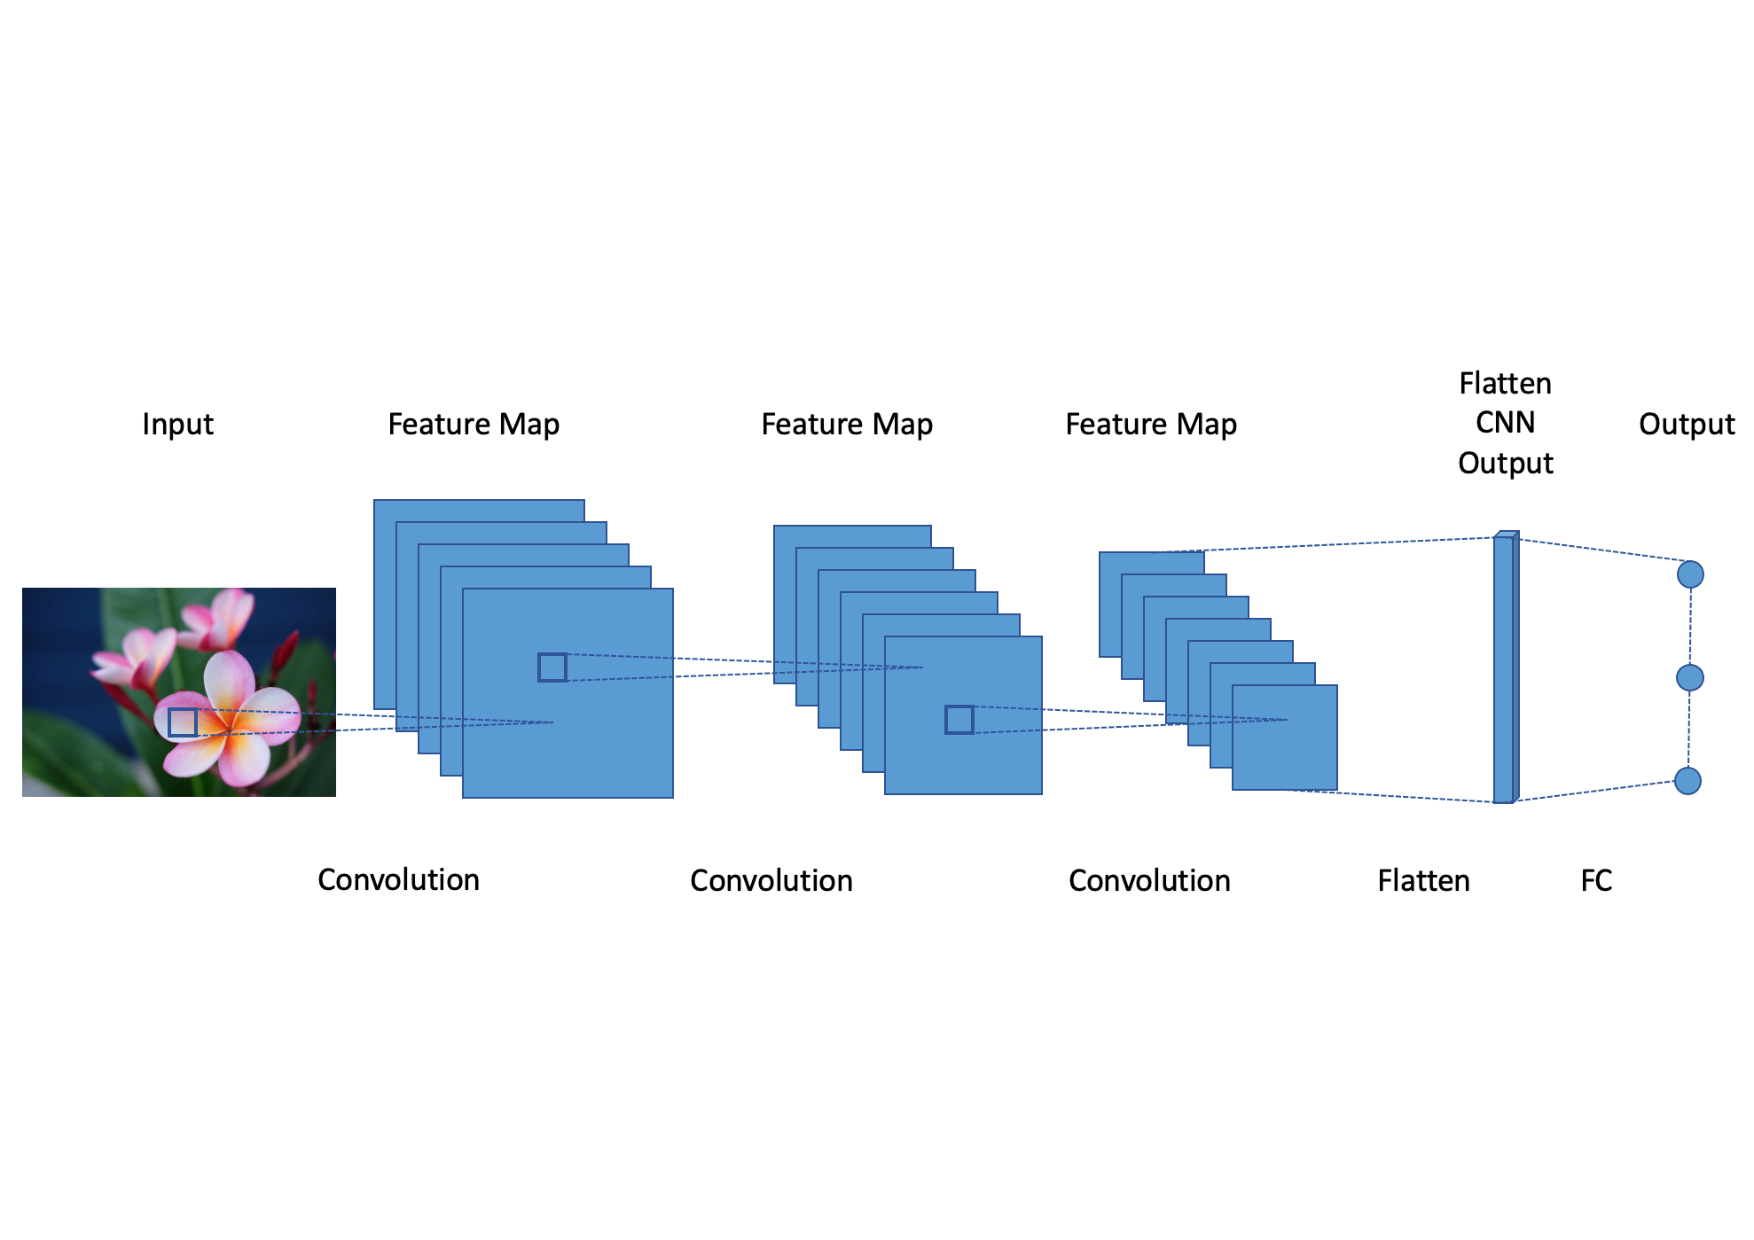
\includegraphics[width=0.9\textwidth]{CNN_overview.pdf}
  \caption {CNN Arcitecture}
  \label{fig:CNN_overview}
\end{figure}


\section{Domain adaptation and Transfer Learning}

\section{Maximum Mean Discrepancy}
Maximum Mean Discrepancy (MMD) is a criterion which estimates the discrepancy between two distribution. MMD can be used to optimize the network such that the distribution discrepancy is reduced in a data domain-invariant feature space. The discrepancy is measured as squared distance between the distribution kernel embeddings in the reproducing kernel Hilbert space (RKHS). The distribution discrepancy across domains is measured in the layers of the neural network in order to avoid feature transferability degradation. One has to pay attention to not transfer noise or irrelevant information. This destroys the structure of the source and target domain data and therefore makes the classification task even more difficult \cite{li2020domain}. 

\begin{align}
    M_{k}(P,Q) = \Bigl|  \boldsymbol{E_{P}}[\Phi(\boldsymbol{X^{s}})] - \boldsymbol{E_{Q}}[\Phi(\boldsymbol{X^{t}})]     \Bigl|^{2}_{Hk}
\end{align}

Hk denotes the RKHS, which is described by the characteristic kernel k and the mapping function $\Phi$. Taking the identity function as mapping function results in matching the distribution means. When using more complex mapping functions also higher order moments can be matched \cite{Yujia2015}. The distributions of the source domain $X^{s} = \{{x}_{i}^{s}\}_{i=0,...,n_{s}}$ and target domain $X^{t} = \{{x}_{i}^{t}\}_{i=0,...,n_{t}}$ are represented by P and Q. $\boldsymbol{E_{p}[.]}$ is the expected value of the source distribution P in the feature space. The kernel choice is of great importance when applying MMD. For this reason it makes sense to combine several kernels in order to profit from their individual performance \cite{li2020domain}.

\begin{align}
    k(\boldsymbol{X^{s}}, \boldsymbol{X^{t}}) = \sum_{i=0}^{N_{k}} k_{\sigma_{i}}(\boldsymbol{X^{s}}, \boldsymbol{X^{t}})
\end{align}

$N_{k}$ denotes the number of kernels used in the the RKHS and $k_{\sigma_{i}}$ represents one individual RBF kernels. Also, other kernels like linear kernels could be used, but current research shows that RBF kernels usually perform best \cite{AZAMFAR2020103932}. In our attempt we used 5 RBF kernels with the bandwidth parameters 1, 2, 4, 8, 16.


